\chapter{Mirkogesten-Erkennung}

Nach der Sichtung der vorgegangen Projektarbeit haben wir uns entschieden, dass zwei Ansätze zur Erkennung der einzelnen Mikrogesten aus der Eingabe-Menge an Punkten im Prototyp ausprobiert und evaluiert werden sollten. Zum einen sollte die in der Projektarbeit favorisierte Erkennung durch die Änderung der Krümmung zwischen den einzelen Punkten getestet werden, zum Anderen ein Ansatz ausprobiert werden, der auf einer auf dem vorausgehenden Punkt basierenden Voraussage des jeweils als nächstes folgenden Punktes aufbaut.

Der Krümmungs-Ansatz wurde in der vorgängigen Projektarbeit neben einem auf der Änderung der Winkel zwischen Punkten basierenden Ansatz zur Mikrogesten-Erkennung evaluiert und am Ende von den Autoren der Arbeit favorisiert. Dadurch war klar, dass wir diese Art der Erkennung ebenfalls für diese Arbeit evaluieren sollten.

Neben einer Erkennung durch die Krümmungs- und die Winkel-Änderung zwischen Punkten sollte unserer Meinung nach auch eine Erkennung durch die Voraussage von folgenden Punkten möglich sein und wurde daher von uns ebenfalls implementiert und evaluiert.

(( TODO Dieser Teil ev. runter ins Fazit))
Als Resultat der Evaluation der beiden genannten Verfahren haben wir uns dazu entschieden, den Ansatz der Erkennung durch die Krümmungs-Änderung weiter zu verfolgen. Während der Evaluation stellte sich heraus dass das auf Voraussagen basierende Verfahren nicht tolerant genug auf kleine Änderungen innerhalb von Mirkogesten reagiert und daher dazu tendiert, diese aufzuteilen. Das Krümmungs-Verfahren wurde von uns als toleranter und daher besser für den mobilen Einsatz geeignet befunden.

\section{Bewertungs-Kriterien}

Kriterium:	Erkennungszuverlässigkeit
Beschreibung:	Um eine verlässliche Erkennung der Mikrogesten zu ermöglichen, muss ein Ansatz natürlich gewährleisten, dass er die Auftrennung der Mirkogesten zuverlässig vornimmt.
Wichtigkeit:	Substantiell

Kriterium:	Toleranz
Beschreibung:	Obwohl die Erkennung natürlich zuverlässig sein sollte, muss aber auch eine gewisse Toleranz für nicht ideale Eingaben gewährt werden. Da die Handschriften-Erkennung auf Menschen und einen Einsatz im mobilen Umfeld ausgerichtet werden soll, sind suboptimale Eingabefolgen durchaus zu erwarten und die Erkennung der Mikrogesten sollte daher einigermassen tolerant auf solche reagieren. Dies stellt offensichtlich ein Zielkonflikt zum Zuverlässigkeits-Kriterium dar und es muss daher ein guter Mittelweg zwischen diesen beiden Kriterien gefunden werden.
Wichtigkeit:	Substantiell

Kriterium:	Performanz
Beschreibung:	Auf einem mobilen System ist der schonende Umgang mit den Systemressourcen besonders wichtig und das Verfahren zur Erkennung der Mikrogesten sollte daher möglichst wenig Rechenleistung brauchen. Da es allerdings nur jeweils nach Benutzereingaben durchgeführt werden muss und eine Ausführung im Hintergrund möglich sein sollte, könnten gewisse Abstriche in diesem Bereich unter Umständen in Kauf genommen werden.
Wichtigkeit:	Sekundär
%================================================
\section{Verfahren zur Auftrennung des Pfades}
\subsection{Ansatz: Punkte-Voraussage}

Grundlage des auf Voraussage des jeweils nächsten Punktes basierenden Ansatzes sollte die Annahme sein, dass man den als nächstes auf einen Punkt einer gleichmässig gekrümmten Kurve folgenden Punkt durch das Spiegeln des jeweils dem Ausgangspunkt vorangehenden Punktes an der Achse des Ausgangspunktes vorherbestimmen können müsste. Weicht der tatsächlich eingegebene Folgepunkt zu sehr vom vorausgesagten Folgepunkt ab, sollte nun angenommen werden, dass dieser Punkt nicht mehr zur aktuellen Mikrogeste gehören und als Ausgangspunkt einer neuen Mikrogeste genommen werden soll.

\subsubsection{Verfahren}

%TODO - Flussdiagramm Prediction-Verfahren

\subsubsection{Bewertung}

Die grundsätzliche Trennung der einzelnen Mikrogesten durch das auf Voraussagen basierende Verfahren wurde von uns als durchaus zufriedenstellend bewertet. Das Verfahren ermöglicht die Auftrennung der Eingabepunkte in verschiedene Mikrogesten. Allerdings erkennt das Verfahren unserer Meinung nach leider zu viele einzelne Mikrogesten und ist zu wenig tolerant gegenüber kleineren Abweichungen. Schon kleinere Änderungen in der Linienführung führen dabei zu einer Auftrennung von ansonsten durchaus zusammenhängenden Gesten.

Auch weist das Verfahren Probleme mit ungleichen Punktedichten auf einem Pfad auf. Dies tritt vor allem auf, wenn die Eingabegeschwindigkeit variiert, etwa wenn nach einer Richtungsänderung oder am Anfang einer Geste die Eingabe beschleunigt wird und die späteren Eingabepunkte weiter auseinander liegen als die ersten. Gerade bei unregelmässigen Beschleunigungen kommt es somit häufig vor, dass die ersten Eingabepunkte relativ nahe beieinander liegen, der Abstand zu späteren Punkten dann aber recht gross wird. Die vorausgesagten Punkte mögen dann zwar durchaus auf dem Pfad der Geste liegen, die Eingabepunkte folgend dann allerdingst erst in grösserem Abstand. Diesem Verhalten könnte möglicherweise mit Anpassungen an der Berechnung der vorausgesagten Punkte begegnet werden. Man könnte etwa anstatt eines konkreten Punktes eine Richtung voraussagen. Auch ein normierter Abstand zwischen den Eingabepunkten, wie ihn das Bezier-Glättungsverfahren erzeugt, welches als mögliche Optimierung in \ref{sec:Glaettung} besprochen wird. Eine Glättung der Eingangspunkte sollte auch die Toleranz des voraussagenden Ansatzes verbessern können.

Weiter haben wir mit diesem Verfahren Probleme mit zu nahe beieinander liegenden Eingabepunkten festgestellt. Ist die Distanz von einem Punkt zum nächsten kleiner als die Länge des Toleranz-Wertes, fällt der Punkt in jedem Fall innerhalb der Toleranz und es kann keine fundierte Aussage über mehr darüber gemacht werden, ob der Punkt zur selben Mirkogeste gehören soll oder nicht. Daher werden nur Punkte, deren Abstand zum Ausgangspunkt kleiner als die zweifache Länge des Toleranz-Wertes sind, beachtet. Andere Punkte werden als zur aktuellen Mikrogeste gehörig angenommen und zum neuen Ausgangspunkt. Dies führt wiederum zu Problemen mit sehr engen Kurven, wie sie etwa bei Richtungswechseln und sehr engwinkligen Spitzen, da diese eng beieinander liegende Eingabepunkte erzeugen, deren Abstand häufig unterhalb die Toleranzgrenze fällt. Somit wird häufig noch der erste Punkt nach einer solchen Spitze zur vorherigen Mikrogeste zugeordnet.

(( TODO diesen Part ev. auf Resultat Sektion verschieben))
Diesen beiden Probleme, welche beide das als substantiell gewertete Bewertungskriterium der Toleranz beinträchtigen, steht steht nur eine gute Performanz durch die relativ simplen Berechnungen, die das Voraussage-Verfahren benötigt, gegenüber. Da das Toleranz-Kriterium von uns aber als signifikant wichtiger eingestuft wurde und vom Krümmungs-Verfahren weit besser erfüllt wird, mussten wir uns am Ende für das auf Krümmungs-Änderungen basierende Verfahren festlegen.

%TODO
%================================================

\subsection{Ansatz: Krümmungs-Änderung}

Das Krümmungsverfahren basiert auf dem Verfahren, das von ((TODO alter Report Referenz einfügen)) vorgeschlagen wird: Die Punkte eines Pfades werden mit Vektoren verbunden. Zwischen jedem Vektor und seinem Nachfolger wird nun das Kreuzprodukt (siehe Abbildung \ref{kreuzprodukt}) gebildet. Das Vorzeichen des Resultats gibt nun die Drehrichtung der Kurve an. Die Änderung der Drehrichtung ist bereits eine wichtige Information um den Pfad in Mikrogesten zu unterteilen.
Als zweite Information erhält man den Winkel zwischen den Vektoren. Nun kann man den Pfad an den Stellen trennen, wo der Winkelunterschied zu den vorherigen Vektoren eine gewisse Toleranz überschreitet. Dies ist vor allem nützlich um zwischen einer starken und einer schwachen Krümmung zu unterscheiden.

\begin{figure}[h!]
  \centering
    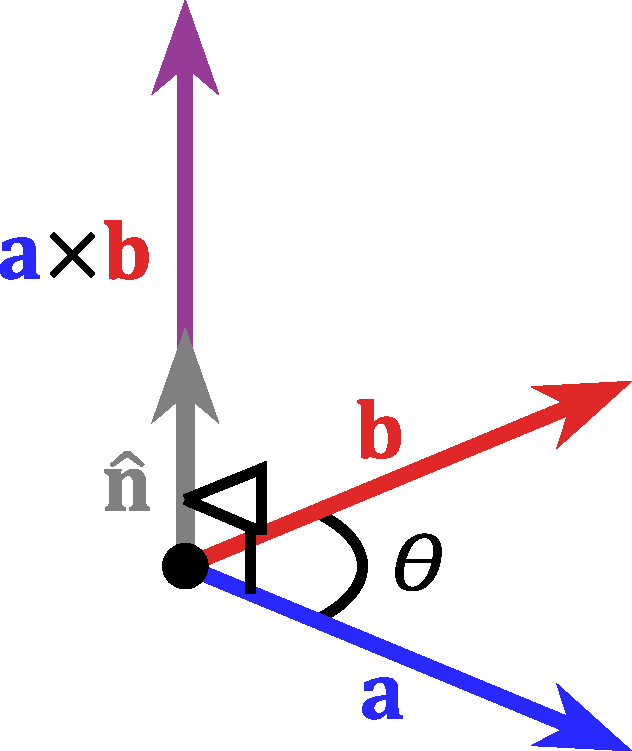
\includegraphics[width=0.3\textwidth]{./img/crossproduct.pdf}
  \caption{Kreuzprodukt zweier Vektoren}
  \label{kreuzprodukt}
\end{figure}

\subsubsection{Verfahren}
Das Vorgehen bei diesem Algorithmus ist sehr simpel: Es wird laufend die Krümmung zwischen dem aktuellen Punkt und seinen Nachbarn berechnet. Sobald die Krümmung einen gewissen Toleranzwert überschreitet wird der Pfad in zwei Mikrogesten aufgetrennt. Der genaue Ablauf ist in Abbildung \ref{curvatureflowchart} ersichtlich.

\begin{figure}[h!]
  \centering
    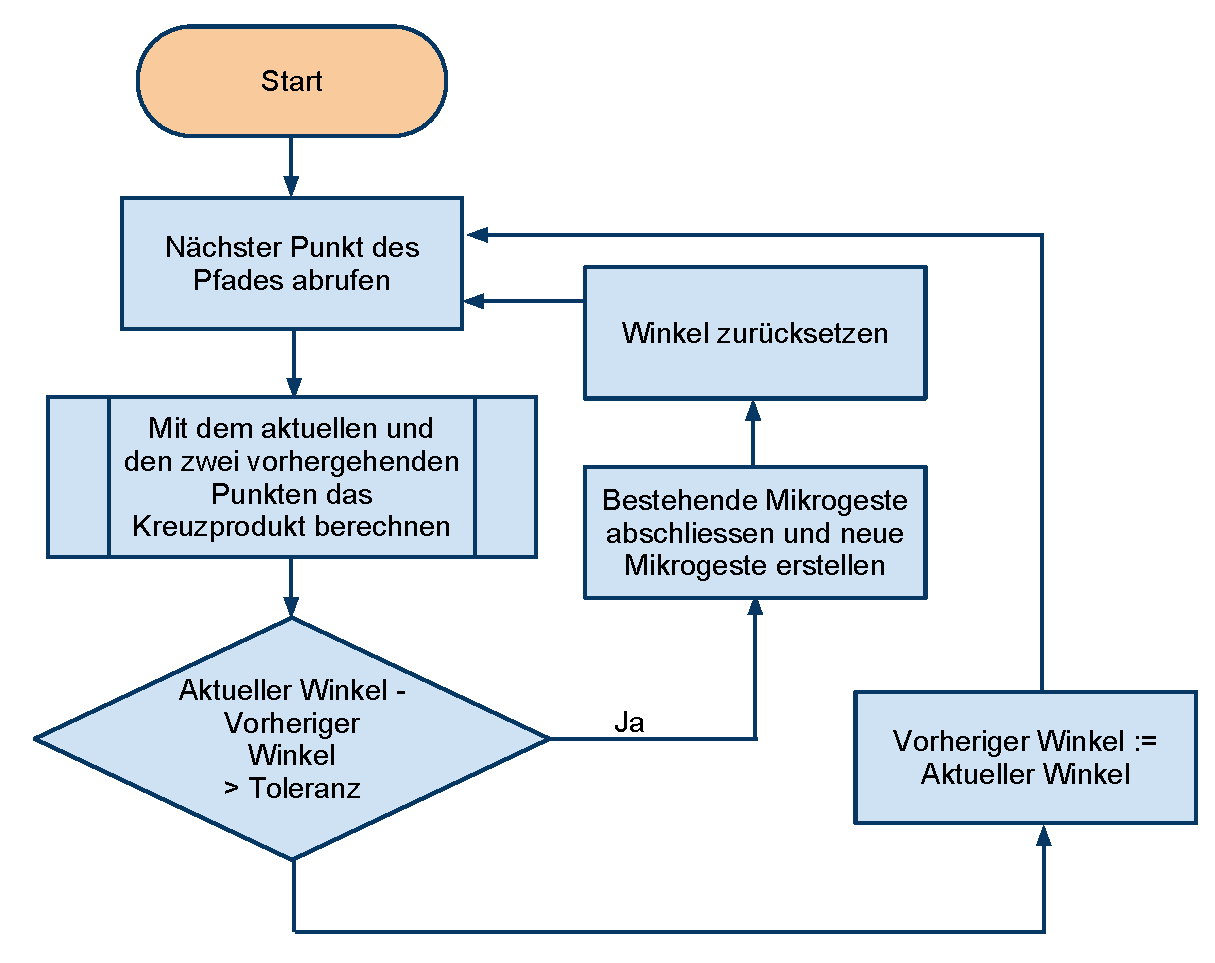
\includegraphics[width=\textwidth]{./img/CurvatureFlowchart.pdf}
  \caption{Ablauf des Krümmungs-Algorithmus}
  \label{curvatureflowchart}
\end{figure}

\subsubsection{Bewertung}
Das Verfahren is vor allem gut geeignet um Änderungen in der Drehrichtung zu erkennen (Nützlich z.B. bei dem Buchstaben 'S') und zwischen starken und schwachen Krümmungen zu unterscheiden. Es hat allerdings die gleichen Probleme wie die Punkte-Voraussage: Die Eingangspunkte müssen gut normiert sein um gleichmässige Erkennung zu garantieren. 

%================================================

\subsection{Ansatz: Drehrichtungs-Erkennung}
Dieser Ansatz ist eine Abwandlung des Krümmungs-Verfahrens und so abgeändert, dass Drehrichtungsänderungen möglichst genau erkannt werden können. Der Hintergedanke dabei ist dass man bei Mikrogesten nur noch zwischen Kurven unterscheidet, die in eine andere Richtung drehen, aber nicht mehr die Stärke der Krümmung berücksichtigt.

\subsubsection{Verfahren}
Das Verfahren funktioniert prinzipiell gleich wie das Krümmungs-Verfahren: Es wird immer für zwei benachbarte Vektoren das Vektorprodukt berechnet. Der errechnete Wert wird immer zu einem Akkumulator addiert und mit dem Punkt abgespeichert. Nach dem der komplette Pfad so durchgerechnet wurde, erhält man eine Akkumulator-Kurve.

\begin{figure}[h!]
  \centering
    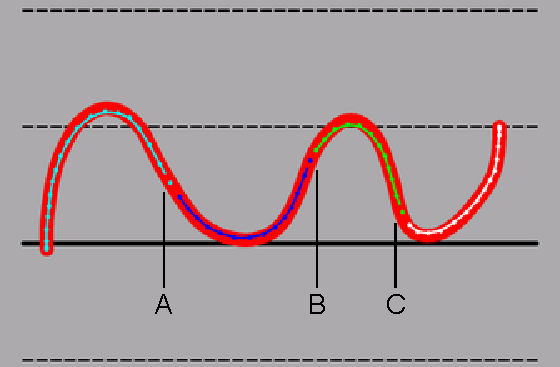
\includegraphics[width=0.67\textwidth]{./img/akkumulator_beispiel.pdf}
  \caption{Beispiel-Eingabe: rot, Erkannte Trennungen: Farbig}
  \label{drehrichtungBeispiel}
\end{figure}

\begin{figure}[h!]
  \centering
    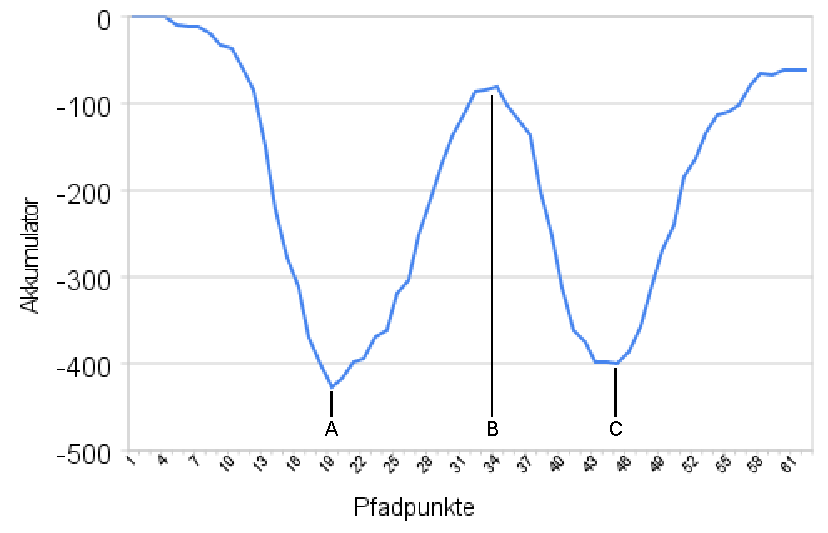
\includegraphics[width=1.0\textwidth]{./img/akkumulator_diagramm.pdf}
  \caption{Akkumulator für die Eingabe von Abbildung \ref{drehrichtungBeispiel}}
  \label{akkumulatorDiagramm}
\end{figure}

\subsubsection{Bewertung}


%================================================

\subsection{Ansatz: Winkel-Änderung}

Dieses Verfahren funktioniert prinzipiell wie das Krümmungs-Verfahren. Es ist jedoch vereinfacht und berücksichtigt nur noch den Winkel zwischen zwei benachbarten Vektoren.

\subsubsection{Verfahren}
Es wird der Winkel zwischen den Vektoren berechnet und mit der Toleranz verglichen. Bei einem genügend spitzigen Winkel wird der Pfad aufgetrennt.

\subsubsection{Bewertung}
Dieses Verfahren ist sehr einfach gehalten und darauf spezialisiert, Spitzkehren im Pfad zu erkennen. Der grosse Nutzen dieses Verfahren ist aber, dass der Pfad nicht normiert werden muss. Die anderen Verfahren erkennen zwar Spitzkehren auch, brauchen aber einen normierten, am besten geglätteten, Pfad. Die Glättung schwächt aber Spitzkehren ab und macht sie ev. sogar unkenntlich.  

%================================================

\subsection{Ansatz: Kreis-Erkennung}
Mit diesem Ansatz sollen alle geschlossenen Kreise auf dem Pfad erkannt werden. Alle restlichen Punkte werden nicht berücksichtigt und müssen mit einem anderen Verfahren aufgetrennt werden.

\subsubsection{Verfahren}
Mit jedem Punkt auf dem Pfad werden alle nachfolgenden Punkte verglichen: Wenn die zwei Punkte sehr nahe beieinander liegen bildet der Pfad zwischen den Punkten ein Kreis.

\begin{lstlisting} [caption={Pseudocode-Algorithmus um Kreise auf einem Pfad zu erkennen},label=kreisalgorithmus]
for(int i=0; i<8;i++) 
{
      //donothing
}
\end{lstlisting}

\subsubsection{Bewertung}
Die Kreiserkennung ist natürlich nur sinnvoll, wenn man eine entsprechende Mikrogeste "Kreis" hat. Allerdings gibt es auch beim Algorithmus noch Verbesserungsbedarf: Bei einem Spezialfall, nämlich ein Pfad der eine '8' bildet, wird der gesamte Pfad als ein Kreis erkannt und nicht als zwei Kreise. 


%================================================
\subsection{Fazit}
Es hat sich gezeigt, dass es nicht sinnvoll ist, sich auf ein einzelnes Verfahren zu stützen. Jedes Verfahren hat seine Schwächen, welche von einem anderen Verfahren abgedeckt werden können. Es ist am besten, den Pfad schrittweise zu unterteilen und bei jedem Schritt die Mikrogesten-Erkennung zu starten. Mit jedem weiteren Schritt werden dann nur noch Pfadteile berücksichtigt, welchen noch keine Mikrogeste zugewiesen ist.

Der Ansatz ist wie folgt:
\begin{enumerate}
	\item Normierung der Punktezahl: Zu nahe beieinander liegende Punkte werden gelöscht. Bei zu grossen Abständen wird zwischen den zwei Punkten interpoliert.
	\item Erkennung der Spitzkehren.
	\item Erkennung aller geschlossenen Kreise 
	\item Unterteilung in Kurven und Geraden
	\item Unterteilung der Kurven bei Drehrichtungswechsel
\end{enumerate}


%================================================

\section{Erkennung der Mikrogesten-Art}

%TODO
%================================================

\section{Erkennung der Ausrichtung einer Mikrogeste}

%TODO
%================================================

\section{Allgemeine Optimierungen}

%TODO

\subsection{Zusammenfügen von minimalen Mikrogesten}

%TODO

\subsection{Glättung der Eingangspunkte}\label{sec:Glaettung}

%TODO - Verschiedene Verfahren, Optimierungen
%================================================

